%Version 3.1 December 2024
% See section 11 of the User Manual for version history
%
%%%%%%%%%%%%%%%%%%%%%%%%%%%%%%%%%%%%%%%%%%%%%%%%%%%%%%%%%%%%%%%%%%%%%%
%%                                                                 %%
%% Please do not use \input{...} to include other tex files.       %%
%% Submit your LaTeX manuscript as one .tex document.              %%
%%                                                                 %%
%% All additional figures and files should be attached             %%
%% separately and not embedded in the \TeX\ document itself.       %%
%%                                                                 %%
%%%%%%%%%%%%%%%%%%%%%%%%%%%%%%%%%%%%%%%%%%%%%%%%%%%%%%%%%%%%%%%%%%%%%

%%\documentclass[referee,sn-basic]{sn-jnl}% referee option is meant for double line spacing

%%=======================================================%%
%% to print line numbers in the margin use lineno option %%
%%=======================================================%%

%%\documentclass[lineno,pdflatex,sn-basic]{sn-jnl}% Basic Springer Nature Reference Style/Chemistry Reference Style

%%=========================================================================================%%
%% the documentclass is set to pdflatex as default. You can delete it if not appropriate.  %%
%%=========================================================================================%%

%%\documentclass[sn-basic]{sn-jnl}% Basic Springer Nature Reference Style/Chemistry Reference Style

%%Note: the following reference styles support Namedate and Numbered referencing. By default the style follows the most common style. To switch between the options you can add or remove "Numbered" in the optional parenthesis. 
%%The option is available for: sn-basic.bst, sn-chicago.bst%  
 
%%\documentclass[pdflatex,sn-nature]{sn-jnl}% Style for submissions to Nature Portfolio journals
%%\documentclass[pdflatex,sn-basic]{sn-jnl}% Basic Springer Nature Reference Style/Chemistry Reference Style
%%\documentclass[pdflatex,sn-mathphys-num]{sn-jnl}% Math and Physical Sciences Numbered Reference Style
%%\documentclass[pdflatex,sn-mathphys-ay]{sn-jnl}% Math and Physical Sciences Author Year Reference Style
%%\documentclass[pdflatex,sn-aps]{sn-jnl}% American Physical Society (APS) Reference Style
\documentclass[pdflatex,sn-vancouver-num]{sn-jnl}% Vancouver Numbered Reference Style (SN Computer Science)
%%\documentclass[pdflatex,sn-vancouver-ay]{sn-jnl}% Vancouver Author Year Reference Style
%%\documentclass[pdflatex,sn-apa]{sn-jnl}% APA Reference Style
%%\documentclass[pdflatex,sn-chicago]{sn-jnl}% Chicago-based Humanities Reference Style

%%%% Standard Packages
%%<additional latex packages if required can be included here>

\usepackage{graphicx}%
\usepackage{multirow}%
\usepackage{amsmath,amssymb,amsfonts}%
\usepackage{amsthm}%
\usepackage{mathrsfs}%
\usepackage[title]{appendix}%
\usepackage{xcolor}%
\usepackage{textcomp}%
\usepackage{manyfoot}%
\usepackage{booktabs}%
\usepackage{algorithm}%
\usepackage{algorithmicx}%
\usepackage{algpseudocode}%
\usepackage{listings}%

%%%% Additional packages required by this manuscript
%%%% (the sn-jnl class already loads "rotating" for sidewaystable)
\usepackage{placeins}%
\usepackage{tikz}%
\usetikzlibrary{arrows.meta,positioning,shapes.geometric}%
%%%%

%%%%%=============================================================================%%%%
%%%%  Remarks: This template is provided to aid authors with the preparation
%%%%  of original research articles intended for submission to journals published 
%%%%  by Springer Nature. The guidance has been prepared in partnership with 
%%%%  production teams to conform to Springer Nature technical requirements. 
%%%%  Editorial and presentation requirements differ among journal portfolios and 
%%%%  research disciplines. You may find sections in this template are irrelevant 
%%%%  to your work and are empowered to omit any such section if allowed by the 
%%%%  journal you intend to submit to. The submission guidelines and policies 
%%%%  of the journal take precedence. A detailed User Manual is available in the 
%%%%  template package for technical guidance.
%%%%%=============================================================================%%%%

%% as per the requirement new theorem styles can be included as shown below
\theoremstyle{thmstyleone}%
\newtheorem{theorem}{Theorem}%  meant for continuous numbers
%%\newtheorem{theorem}{Theorem}[section]% meant for sectionwise numbers
%% optional argument [theorem] produces theorem numbering sequence instead of independent numbers for Proposition
\newtheorem{proposition}[theorem]{Proposition}% 
%%\newtheorem{proposition}{Proposition}% to get separate numbers for theorem and proposition etc.

\theoremstyle{thmstyletwo}%
\newtheorem{example}{Example}%
\newtheorem{remark}{Remark}%

\theoremstyle{thmstylethree}%
\newtheorem{definition}{Definition}%

\raggedbottom
%%\unnumbered% uncomment this for unnumbered level heads

\begin{document}


%%==================================%%
%%               Title              %%
%%==================================%%

\title[CPARMS-WMF]{
CPARMS-WMF: Clustering and Pairwise Association Rule Mining Signal for WMF with Sparse Implicit Feedback
}


%%==================================%%
%%               Name               %%
%%==================================%%

%%=============================================================%%
%% GivenName	-> \fnm{Joergen W.}
%% Particle	-> \spfx{van der} -> surname prefix
%% FamilyName	-> \sur{Ploeg}
%% Suffix	-> \sfx{IV}
%% \author*[1,2]{\fnm{Joergen W.} \spfx{van der} \sur{Ploeg} 
%%  \sfx{IV}}\email{iauthor@gmail.com}
%%=============================================================%%
\author[1]{\fnm{Peerapat} \sur{Tancharoen}\orcid{https://orcid.org/0009-0009-9937-5382}}\email{peerapat.tcr@gmail.com}

\author[2]{\fnm{Bussaba} \sur{Amnueypornsakul}}\email{bussaba.a@kbtg.tech}

\author*[1]{\fnm{Arit} \sur{Thammano}}\email{arit@it.kmitl.ac.th}

\affil*[1]{\orgdiv{Artificial Intelligence for Business Analytics},
\orgname{School of Information Technology, King Mongkut's Institute of Technology Ladkrabang},
\orgaddress{\city{Bangkok}, \postcode{10520}, \country{Thailand}}}

\affil[2]{\orgname{KASIKORN Business-Technology Group},
\orgaddress{\city{Pak Kret}, \state{Nonthaburi}, \postcode{11120}, \country{Thailand}}}


%%==================================%%
%%             Abstract             %%
%%==================================%%

\abstract{
Weighted matrix factorization (WMF) struggles when interactions are sparse and side information is not always available. We investigate whether patterns derived only from the interaction matrix can improve personalized Top-$K$ recommendation for users with short positive histories.

We propose CPARMS-WMF, a feature-free framework that clusters users and items from positive feedback, mines single-antecedent rules over user-cluster, liked-item-cluster, and item-level tokens, and incorporates the resulting user--item scores into WMF. We evaluate it on five Amazon datasets using a global temporal split and five random seeds against MostPop, Standard-WMF, and CoFactor-WMF.

CPARMS-WMF wins $73/75$ dataset--seed baseline comparisons: $25/25$ against MostPop and $24/25$ against each WMF baseline. Its mean normalized discounted cumulative gain at cutoff 10 (NDCG@10) is highest on all five datasets. For one-interaction users, it wins $21/25$ comparisons against Standard-WMF, $19/25$ against CoFactor-WMF, and $13/25$ against MostPop.

CPARMS-WMF improves ranking over both WMF baselines overall and in most comparisons for one-interaction users, but popularity remains competitive.
}

\keywords{ Recommender systems, Sparse implicit feedback, Weighted matrix factorization, Clustering, Association rule mining }

%%\pacs[JEL Classification]{D8, H51}

%%\pacs[MSC Classification]{35A01, 65L10, 65L12, 65L20, 65L70}

\maketitle


%%==================================%%
%% Introduction %%
%%==================================%%

\section{Introduction}\label{sec1}

Recommender systems help people find relevant products and content in large catalogs, but recommendation quality often decreases for users with only one or a few recorded interactions.

Collaborative filtering, especially matrix factorization (MF) \cite{koren2009mf}, remains widely used for its accuracy and scalability; it learns directly from interaction data, without requiring any side information. Weighted matrix factorization (WMF) \cite{hu2008implicit} adapts MF to implicit feedback by assigning different confidence levels to observed and unobserved interactions. Alternating least squares (ALS) can optimize it efficiently. Both MF and WMF still need enough interaction history: when a user's history contains only a few interactions, the corresponding latent factors cannot be estimated reliably, and Top-$K$ ranking quality drops; highly sparse datasets make this even worse \cite{roy2022systematic}.

One common solution to user sparsity is to add side information such as user profiles, demographic attributes, item descriptions, or cross-domain knowledge \cite{nguyen2013contentBoostedMF,fernandezTobias2019crossDomainColdStart,parthasarathy2023hybrid}. Side information can improve accuracy, but it is not always available. This gap motivates feature-free methods, which do not require user attributes or item metadata.

The interaction matrix contains patterns beyond the history of any single user or item. Clustering can reveal group-level preferences \cite{mirbakhsh2016leveraging}, and item co-occurrence can strengthen latent-factor learning \cite{liang2016cofactor}. Association rule mining can reveal directional relationships: previous work has combined item clustering with association rule mining to reduce sparsity \cite{najafabadi2017clusteringARM}, and CFCAI applies cluster-level rule mining to cold-start recommendation \cite{khaledian2025cfcai}.

These studies motivate integrating clustering, association rule mining, and weighted matrix factorization in a single model. Clustering captures shared preference structure, association rules identify directional relationships, and WMF uses this information for personalized ranking. CPARMS-WMF combines these signals within a single objective.

We propose \textbf{CPARMS-WMF}, a feature-free framework for personalized recommendation under sparse implicit feedback. Its \textbf{Clustering and Pairwise Association Rule Mining Signal (CPARMS)} is derived only from the user--item interaction matrix. CPARMS clusters users and items by positive interaction patterns, mines single-antecedent rules from user-cluster, liked-item-cluster, and item-level tokens, and converts those rules into a user--item signal. An additional CPARMS term incorporates this signal into the ALS objective.

We evaluate only users and items observed in the fit window. Users and items that appear only in the evaluation window are excluded from training and the candidate set, and their evaluation events are not scored. Among the remaining users, we include only those with at least one positive interaction in the fit window and at least one positive target in the evaluation window. Results are reported overall and separately for users with one, two, and three or more positive interactions.

CPARMS-WMF is compared with three feature-free baselines: a non-personalized popularity baseline (MostPop), Standard-WMF, and CoFactor-WMF.

The main contributions are:

\begin{enumerate}
\item CPARMS-WMF is introduced as a feature-free method for recommendation under sparse implicit feedback that does not require user attributes or item metadata.

\item CPARMS combines user and item clustering with pairwise association rule mining. It mines user-cluster, liked-item-cluster, and item-level rules from the transactions.

\item CPARMS is integrated into WMF through an additional CPARMS term optimized by alternating least squares.

\item CPARMS-WMF is evaluated on five Amazon domains using five random seeds. NDCG@10 is the primary metric, with NDCG@20, NDCG@50, NDCG@100, and NDCG@200 reported as secondary measures. The analysis covers mean performance and pairwise dataset--seed comparisons against all three baselines, both overall and for users with one, two, and three or more positive interactions. It also identifies where CPARMS-WMF improves over the WMF baselines and where popularity remains competitive.
\end{enumerate}

%%==================================%%
%%          related work           %%
%%==================================%%

\section{Related Work}\label{sec2}

We first review matrix factorization for implicit feedback and then consider feature-free methods that extract additional structure from the interaction matrix.

\subsection{Matrix Factorization and Weighted Matrix Factorization}

Matrix factorization (MF) is a core recommendation technique. It places users and items in a shared low-dimensional latent space and estimates preferences from how their latent factors interact \cite{koren2009mf}.

Weighted matrix factorization (WMF) extends MF to implicit-feedback data by modeling binary preference alongside confidence weights. WMF learns its latent factors by minimizing a confidence-weighted WMF loss, most often with alternating least squares \cite{hu2008implicit}.

Both methods remain sensitive to sparsity: when observed interactions are limited, estimates become unreliable, and Top-$K$ ranking quality drops \cite{roy2022systematic}. This problem motivates additional signals derived from interactions.

\subsection{Non-personalized Recommendation}

Ranking candidate items by global popularity, identically for every user, is the standard non-personalized reference point in recommender evaluation \cite{aggarwal2016recommender,zangerle2022fevr}. Because this baseline does not use individual user histories, a personalized model that cannot outperform it has not demonstrated an accuracy benefit from personalization under this evaluation protocol. Popularity remains a strong Top-$N$ baseline: prior work shows that a naive TopPop method can rival sophisticated personalized algorithms and that highly popular items can skew Top-$N$ accuracy \cite{cremonesi2010performance}. Section~\ref{sec5} shows that it outperforms Standard-WMF on two of our five datasets.

\subsection{Hybrid Matrix Factorization with Side Information}

A common approach to reducing sparsity is to use side information with collaborative filtering. Content-boosted matrix factorization adds item attributes directly to the factorization, improving predictive accuracy and making recommendations easier to interpret \cite{nguyen2013contentBoostedMF}.

Cross-domain matrix factorization transfers information from related domains by using item metadata and semantic relationships as links between source and target items. It is especially helpful for new users \cite{fernandezTobias2019crossDomainColdStart}. More broadly, hybrid recommender systems combine collaborative and content-based filtering so that each approach can address the weaknesses of the other \cite{parthasarathy2023hybrid}.

\subsection{Hybrid Matrix Factorization without Side Information}

Interaction-derived methods draw additional signals from user--item data without requiring external attributes. Clustering-based approaches identify preference structures shared by users or items \cite{mirbakhsh2016leveraging}, while association-rule approaches mine directional item relationships from transaction data. Some studies combine the two techniques or connect one of them to matrix factorization. For example, one approach reduces the dimensionality of the item space through clustering and then applies association rule mining to implicit interactions \cite{najafabadi2017clusteringARM}. CFCAI mines rules between clusters to support cold-start recommendation, while also using demographic and profile information \cite{khaledian2025cfcai}. CoFactor instead adds an item--item co-occurrence term to the factorization objective, supplying information for items with few observed interactions \cite{liang2016cofactor}. To our knowledge, none of the studies reviewed above integrates clustering, association rule mining, and weighted matrix factorization within one model.

CoFactor is a relevant weighted matrix factorization baseline because it links implicit-feedback WMF with an item--item co-occurrence signal derived from the same interaction matrix \cite{liang2016cofactor}. CoFactor-WMF augments Standard-WMF with an item--item shifted positive pointwise mutual information (SPPMI) term. Using the notation of this paper, a CoFactor-style objective is
\begin{equation}
\begin{aligned}
\mathcal{L}_{\mathrm{CoFactor}}
=&
\sum_{u\in\mathcal{U}}\sum_{i\in\mathcal{I}}
c_{ui}
\left(
\pi_{ui}-\mathbf{p}_u^{\top}\mathbf{q}_i
\right)^2 \\
&+
\gamma_{\mathrm{co}}
\sum_{(i,j)\in\mathcal{M}}
\left(
m_{ij}
-\mathbf{q}_i^{\top}\mathbf{z}_j
-b_i-d_j
\right)^2 \\
&+
\lambda
\left(
\lVert\mathbf{P}\rVert_F^2+
\lVert\mathbf{Q}\rVert_F^2
\right)
+
\lambda_{\mathrm{ctx}}\lVert\mathbf{Z}\rVert_F^2 .
\end{aligned}
\label{eq:cofactor_objective}
\end{equation}
Here $\pi_{ui}$ is the binary implicit preference, $c_{ui}$ is its WMF confidence weight, $\mathbf{p}_u$ and $\mathbf{q}_i$ are user and item factors, $m_{ij}$ is the SPPMI value for item $i$ and context item $j$, $\mathcal{M}$ indexes nonzero SPPMI entries, $\mathbf{z}_j$ is a context factor, $b_i$ and $d_j$ are item-side and context-side biases, $\gamma_{\mathrm{co}}$ controls the co-occurrence-term weight, and $\lambda_{\mathrm{ctx}}$ regularizes the context factors. The shared item factor $\mathbf{q}_i$ connects the WMF term to the SPPMI term. We compute the SPPMI entries from item co-occurrence counts $c_{ij}$, where $c_{ij}$ is the number of users who positively interacted with both items $i$ and $j$, and we set the diagonal to zero:
\begin{equation}
\operatorname{SPPMI}_{ij}
=
\max\left(
\log
\frac{c_{ij}N}{f_i f_j}
-
\log k,
0
\right),
\label{eq:sppmi}
\end{equation}
where $N$ is the total co-occurrence count over nonzero entries, $f_i$ and $f_j$ are the marginal co-occurrence counts of items $i$ and $j$, and $k$ is the number of negative samples, whose logarithm shifts the pointwise mutual information. CoFactor therefore adds a signal derived from interactions, but this signal encodes item-level co-occurrence rather than group-level user preference patterns.

Equation~\eqref{eq:cofactor_objective} keeps the co-occurrence term weighted and the WMF term at unit scale. The original formulation instead applies a relative scale $\ell$ to the WMF term and its user and item regularizers. Dividing the objective by $\ell$ gives Eq.~\eqref{eq:cofactor_objective} with $\gamma_{\mathrm{co}}=1/\ell$ and $\lambda_{\mathrm{ctx}}=\gamma_{\mathrm{co}}\lambda$. Our implementation and hyperparameter search keep this relationship: we sample $\ell$ and derive $\gamma_{\mathrm{co}}$ and $\lambda_{\mathrm{ctx}}$ from it (Section~\ref{sec4_hyperparameter}).

\subsection{How the Proposed Method Differs}

The feature-free methods reviewed above use one or two of clustering, association rule mining, and weighted matrix factorization. CPARMS-WMF combines all three in one framework: clustering provides group-level preference structure shared across the members of each user or item cluster, pairwise association rules provide directional confidence-weighted information, and WMF provides personalized latent-factor ranking. CoFactor-WMF adds SPPMI item co-occurrence to matrix factorization, which makes it a suitable baseline for CPARMS-WMF because both use extra information from the interaction matrix. The main difference is that CoFactor-WMF regularizes shared item embeddings with item-level co-occurrence, while CPARMS builds a user--item signal from item--item, user-cluster--item, and liked-item-cluster--item relations.

CPARMS uses three token families: user-cluster, liked-item-cluster, and item-level tokens. User-cluster tokens provide a generic signal shared by users in the same cluster, while the other two provide personalized signals based on each user's positive history.

This comparison raises two questions. First, can CPARMS-WMF improve personalized ranking under sparse implicit feedback, beating Standard-WMF, CoFactor-WMF, and the non-personalized popularity baseline? Second, does this improvement remain for users with extremely short histories, including when compared with the popularity baseline? The results in Section~\ref{sec5} support the first claim but only partly support the second.


%%==================================%%
%%          proposed method         %%
%%==================================%%

\section{Proposed Method}\label{sec3}

\textbf{CPARMS-WMF} is designed to improve Top-$K$ recommendation under sparse implicit feedback by deriving its CPARMS signal through clustering and pairwise association rule mining on the user--item interaction matrix.

Three main components make up the framework: (i) interaction-based clustering of users and items, followed by pairwise association rule mining; (ii) construction of a sparse user--item recommendation signal from the rules; and (iii) integration of that signal into a weighted matrix factorization objective optimized by alternating least squares.

\subsection{Notation and Feedback Views}

Let $\mathcal{U}=\{1,\ldots,U\}$ and $\mathcal{I}=\{1,\ldots,I\}$ be the user and item index sets, and let $\mathbf{Y}=[y_{ui}] \in \mathbb{R}_{\ge 0}^{U \times I}$ be the interaction matrix of the fit window. From $\mathbf{Y}$ the pipeline derives two binary views and keeps them strictly separate:
\begin{equation}
\underbrace{b_{ui} = \mathbb{I}\!\left[\, y_{ui} > 0 \,\right]}_{\textstyle \mathbf{B}\;(\text{seen})},
\qquad
\underbrace{\ell_{ui} = \mathbb{I}\!\left[\, y_{ui} > \theta \,\right]}_{\textstyle \mathbf{L}\;(\text{liked})},
\qquad \theta=3.
\label{eq:binary}
\end{equation}
$\mathbf{L}$ is the positive feedback (``liked'') view: at $\theta=3$, integer ratings of four or higher count as positive. This threshold follows the MovieLens preprocessing used in CoFactor~\cite{liang2016cofactor}. We additionally retain $\mathbf{B}$ as the ``seen'' view, recording every observed rating at any level so that all previously rated items can be masked at ranking time.

All learned inputs are derived from $\mathbf{L}$: the cluster assignments, transaction tokens, association rules, SPPMI matrix, and WMF preference target. The matrix $\mathbf{B}$ is used only to mask candidates. An item is therefore treated as seen after any rating, even one below the like threshold, and is not recommended again. For user $u$, let $\Omega_u^{+}=\{i \mid \ell_{ui}=1\}$ denote the positive history, $\Omega_u=\{i \mid b_{ui}=1\} \supseteq \Omega_u^{+}$ the seen set, and $n_u=|\Omega_u^{+}|$.


\subsection{CPARMS: Clustering and Pairwise Association Rule Construction}

Previous studies show that clustering and association rule mining can improve collaborative filtering on sparse data~\cite{mirbakhsh2016leveraging,najafabadi2017clusteringARM}. CPARMS builds on these ideas to construct an additional sparse signal using only positive interactions.

We cluster users and items separately with K-means~\cite{macqueen1967kmeans} on the binary positive feedback matrix. Each fit uses K-means++ initialization, $10$ restarts, and the experiment seed. K-means is fitted only to active rows, which contain at least one positive interaction, and the fitted model then assigns every row---including an all-zero row---to its nearest cluster. Excluding all-zero rows from fitting prevents identical inactive rows from forming an uninformative cluster. User clustering operates on the rows of $\mathbf{L}$ and produces $K_U$ clusters; the one-hot matrix $\mathbf{U} \in \{0,1\}^{U \times K_U}$ records each user's assignment. Item clustering operates on the rows of $\mathbf{L}^{\top}$ and produces the one-hot assignment matrix $\mathbf{G} \in \{0,1\}^{I \times K_I}$. We then construct a binary liked-item-cluster matrix that records whether a user's positive history contains any item from each cluster:
\begin{equation}
\mathbf{E} = \mathbb{I}\!\left[\, \mathbf{L}\mathbf{G} > 0 \,\right] \in \{0,1\}^{U \times K_I}.
\label{eq:presence}
\end{equation}
When $K_U=1$, all users share the same user-cluster token, which acts as a dataset-wide popularity signal. Validation selects this setting for some datasets (Section~\ref{sec5}).

For each user, we stack three token families (user-cluster tokens, liked-item-cluster tokens, and item-level tokens) into a single transaction matrix:
\begin{equation}
\mathbf{T} = \big[\, \mathbf{L} \;\big|\; \mathbf{U} \;\big|\; \mathbf{E} \,\big]
\in \{0,1\}^{U \times M}, \qquad M = I + K_U + K_I .
\label{eq:tokens}
\end{equation}
Let $\mathcal{A}$ index all $M$ tokens, and let $\mathcal{R}$ be the item-level tokens, which are the only valid consequents. We use user-cluster and liked-item-cluster tokens only as antecedents, so every rule has an individual item as its consequent.

We mine single-antecedent directed rules from joint token counts. Given the pair-count matrix $\mathbf{C} = \mathbf{T}^{\top}\mathbf{T}$ and token frequency $n_t = \sum_{u} T_{ut}$, the metrics for a rule $a \rightarrow b$ are:
\begin{equation}
\mathrm{sup}(a \rightarrow b) = \frac{C_{ab}}{U}, \quad
\mathrm{conf}(a \rightarrow b) = \frac{C_{ab}}{n_a}, \quad
\mathrm{lift}(a \rightarrow b) = \frac{U \, C_{ab}}{n_a \, n_b}.
\label{eq:metrics}
\end{equation}
Confidence is the conditional probability that a user linked to antecedent $a$ is also linked to consequent $b$, and therefore measures the rule's directional reliability. Lift compares the joint frequency with that expected under independence: $\mathrm{lift}>1$ indicates a positive association beyond chance, whereas $\mathrm{lift}\approx 1$ indicates a relationship already explained by the consequent's overall popularity. We consider only directional pairs with $a \neq b$ and $b \in \mathcal{R}$. A rule is selected when it meets the configured minimum support, confidence, and lift. All three thresholds are tuned on validation data (Section~\ref{sec4_hyperparameter}). The rule-selection indicator is
\begin{equation}
D_{ab} = \mathbb{I}\!\left[\,
\mathrm{sup}(a \rightarrow b) \ge \sigma_{\min} \;\land\;
\mathrm{conf}(a \rightarrow b) \ge \rho_{\min} \;\land\;
\mathrm{lift}(a \rightarrow b) \ge \ell_{\min}
\,\right].
\label{eq:mask}
\end{equation}
Each selected rule keeps its confidence as its weight:
\begin{equation}
W_{ab} = D_{ab}\,\mathrm{conf}(a \rightarrow b).
\label{eq:rule_weight}
\end{equation}
Thus, retained rules carry weight in proportion to their directional reliability, while support and lift serve only as noise filters through Eq.~\eqref{eq:mask}. Collecting the retained rules produces $\mathbf{W} \in \mathbb{R}^{M \times I}$, which encodes the filtered relationships from antecedent tokens to individual-item consequents.

\begin{figure}[t]
\centering
\resizebox{\textwidth}{!}{%
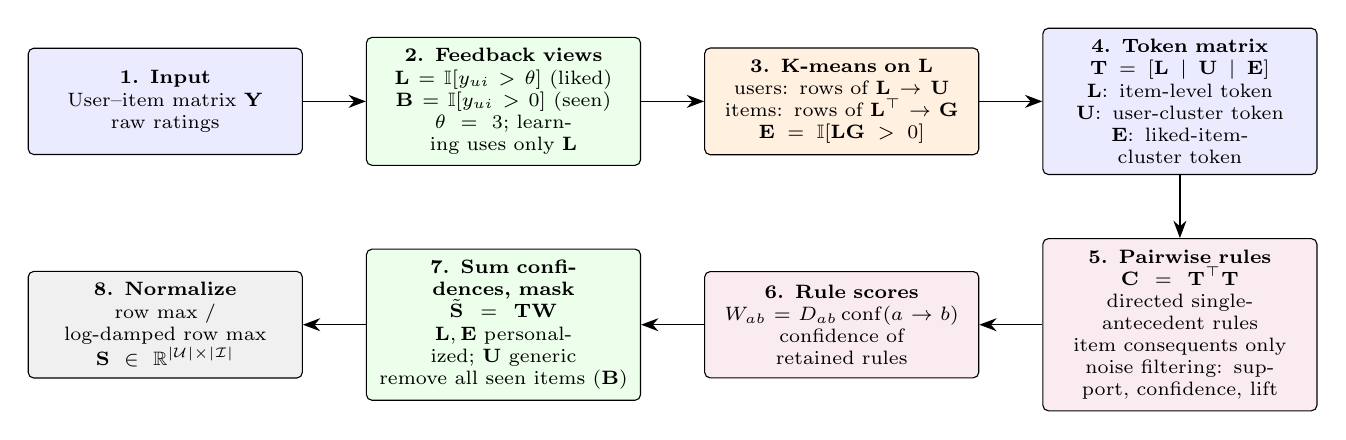
\begin{tikzpicture}[
    font=\scriptsize,
    node distance=8mm and 8mm,
    stage/.style={draw, rounded corners=2pt, align=center, text width=3.2cm, minimum height=1.35cm, inner sep=4pt},
    matrixstage/.style={stage, fill=blue!8},
    transformstage/.style={stage, fill=green!8},
    clusterstage/.style={stage, fill=orange!12},
    rulestage/.style={stage, fill=purple!8},
    outputstage/.style={stage, fill=gray!12},
    arrow/.style={-{Stealth[length=2.2mm]}, line width=0.45pt}
]
\node[matrixstage] (s1) {\textbf{1. Input}\\User--item matrix $\mathbf{Y}$\\raw ratings};
\node[transformstage, right=of s1] (s2) {\textbf{2. Feedback views}\\$\mathbf{L}=\mathbb{I}[y_{ui}>\theta]$ (liked)\\$\mathbf{B}=\mathbb{I}[y_{ui}>0]$ (seen)\\$\theta=3$; learning uses only $\mathbf{L}$};
\node[clusterstage, right=of s2] (s3) {\textbf{3. K-means on $\mathbf{L}$}\\users: rows of $\mathbf{L}\rightarrow\mathbf{U}$\\items: rows of $\mathbf{L}^{\top}\rightarrow\mathbf{G}$\\$\mathbf{E}=\mathbb{I}[\mathbf{L}\mathbf{G}>0]$};
\node[matrixstage, right=of s3] (s4) {\textbf{4. Token matrix}\\$\mathbf{T}=[\mathbf{L}\mid\mathbf{U}\mid\mathbf{E}]$\\$\mathbf{L}$: item-level token\\$\mathbf{U}$: user-cluster token\\$\mathbf{E}$: liked-item-cluster token};
\node[rulestage, below=of s4] (s5) {\textbf{5. Pairwise rules}\\$\mathbf{C}=\mathbf{T}^{\top}\mathbf{T}$\\directed single-antecedent rules\\item consequents only\\noise filtering: support, confidence, lift};
\node[rulestage, left=of s5] (s6) {\textbf{6. Rule scores}\\$W_{ab}=D_{ab}\,\mathrm{conf}(a\rightarrow b)$\\confidence of retained rules};
\node[transformstage, left=of s6] (s7) {\textbf{7. Sum confidences, mask}\\$\tilde{\mathbf{S}}=\mathbf{T}\mathbf{W}$\\$\mathbf{L},\mathbf{E}$ personalized; $\mathbf{U}$ generic\\remove all seen items ($\mathbf{B}$)};
\node[outputstage, left=of s7] (s8) {\textbf{8. Normalize}\\row max /\\log-damped row max\\$\mathbf{S}\in\mathbb{R}^{|\mathcal{U}|\times|\mathcal{I}|}$};
\draw[arrow] (s1) -- (s2);
\draw[arrow] (s2) -- (s3);
\draw[arrow] (s3) -- (s4);
\draw[arrow] (s4) -- (s5);
\draw[arrow] (s5) -- (s6);
\draw[arrow] (s6) -- (s7);
\draw[arrow] (s7) -- (s8);
\end{tikzpicture}%
}
\caption{Overview of the CPARMS signal-generation pipeline, from the raw user--item
interaction matrix~$\mathbf{Y}$ to the normalized user--item signal matrix~$\mathbf{S}$.
All learning happens on the liked view~$\mathbf{L}$; the seen view~$\mathbf{B}$ enters only
as the candidate mask in stage~7}
\label{fig:cparms_pipeline}
\end{figure}

\subsection{CPARMS Signal Generation}

Figure~\ref{fig:cparms_pipeline} summarizes the implemented pipeline. CPARMS produces two sources of information. Rules triggered by user-cluster tokens in $\mathbf{U}$ give a generic score shared by members of the same cluster. Rules triggered by liked-item-cluster tokens in $\mathbf{E}$ or item-level tokens in $\mathbf{L}$ give personalized scores because both token types depend on the user's own positive history.

To form the raw signal, CPARMS applies the rule scores in $\mathbf{W}$ to every token in a user's transaction row, summing, for each candidate item, the scores of all rules triggered by the user's active tokens:
\begin{equation}
\tilde{\mathbf{S}} = \mathbf{T}\,\mathbf{W} \;\in\; \mathbb{R}^{U \times I}.
\label{eq:signal_raw}
\end{equation}
Because the token families occupy separate column blocks of $\mathbf{T}$, this sum divides exactly into the two types of information. We define
\begin{equation}
\mathbf{T}^{(p)} = \big[\, \mathbf{L} \;\big|\; \mathbf{0}_{U\times K_U} \;\big|\; \mathbf{E} \,\big],
\qquad
\mathbf{T}^{(g)} = \big[\, \mathbf{0}_{U\times I} \;\big|\; \mathbf{U} \;\big|\; \mathbf{0}_{U\times K_I} \,\big].
\end{equation}
The raw signal is the equal-weight sum of the personalized and generic signals:
\begin{equation}
\tilde{\mathbf{S}}
= \mathbf{T}^{(p)}\mathbf{W} + \mathbf{T}^{(g)}\mathbf{W}
= \tilde{\mathbf{S}}^{(p)} + \tilde{\mathbf{S}}^{(g)} .
\label{eq:signal_sum}
\end{equation}
There is no specific blending parameter; the way the two signals combine depends entirely on token activation. Every user activates one user-cluster token, so the generic signal gives a shared cluster-level score vector to each cluster member. In contrast, the number of active personalized antecedents grows with $n_u$, so the personalized signal becomes stronger as positive history grows.

Equation~\eqref{eq:signal_sum} shows that a user with $n_u=0$ would receive only the generic signal. We do not evaluate this case because users with no positive interactions are outside the evaluation population (Section~\ref{sec4_split}).

After summing the confidence scores, we set the score of every seen item to zero using $\mathbf{B}$, so the signal applies only to unseen items. Since the seen set includes all positive items, none of them retains a signal score.

The unseen signal is then normalized using one of two searched modes. Row-wise maximum scaling divides each user row by its own maximum. Log-transformed row-wise scaling first compresses heavy-tailed rule-score sums with $\log(1+\cdot)$ so that a single dominant item does not compress the remaining scores in the row toward zero. Let $\tilde{s}_{ui}$ be the unseen raw signal. The two modes are:
\begin{equation}
s_{ui} = \frac{\tilde{s}_{ui}}{\max_{j}\tilde{s}_{uj}},
\qquad\text{or}\qquad
s_{ui} = \frac{\log\!\big(1+\tilde{s}_{ui}\big)}{\max_{j}\log\!\big(1+\tilde{s}_{uj}\big)}.
\label{eq:normalize}
\end{equation}
Empty rows remain zero, and $0 \le s_{ui} \le 1$ under either mode. This yields the sparse, non-negative CPARMS signal matrix $\mathbf{S} = [s_{ui}] \in \mathbb{R}_{\ge 0}^{U \times I}$. We write $\Psi_u = \{\, i \mid s_{ui} > 0 \,\}$ for each user's set of signal-supported items; by construction, $\Psi_u \cap \Omega_u = \varnothing$.

\subsection{CPARMS-WMF: Signal-Regularized Weighted Matrix Factorization}

CPARMS-WMF integrates the signal into a single matrix factorization objective. It adds a CPARMS term over signal-supported items to implicit-feedback WMF~\cite{hu2008implicit}, similar to the additional SPPMI term in CoFactor~\cite{liang2016cofactor}. We compute interaction scores as the inner product of latent factors:
\begin{equation}
\hat{y}_{ui} = \mathbf{p}_u^{\top}\mathbf{q}_i,
\qquad \mathbf{p}_u, \mathbf{q}_i \in \mathbb{R}^{K},
\label{eq:mf_pred}
\end{equation}
where $K$ is the latent dimension. Stacking row-wise gives $\mathbf{P}\in\mathbb{R}^{U\times K}$ and $\mathbf{Q}\in\mathbb{R}^{I\times K}$. The preference target is the liked view of Eq.~\eqref{eq:binary}, and every pair gets an implicit-feedback confidence that up-weights positives,
\begin{equation}
\pi_{ui} = \ell_{ui},
\qquad
c_{ui} = 1 + \alpha\,\pi_{ui},
\label{eq:pref_conf}
\end{equation}
where $\alpha \ge 0$ sets the extra confidence placed on positive interactions. One threshold $\theta=3$ defines positives across CPARMS construction, SPPMI construction, WMF training, and evaluation relevance.

The training objective combines a confidence-weighted WMF term over all user--item pairs, a $\gamma$-weighted CPARMS term over signal-supported pairs, and an $\ell_2$ penalty,
\begin{equation}
\begin{aligned}
\mathcal{L} =\;
& \sum_{u\in\mathcal{U}}\sum_{i\in\mathcal{I}}
c_{ui}\,\big(\pi_{ui} - \hat{y}_{ui}\big)^2
\;+\;
\gamma \sum_{u\in\mathcal{U}}\sum_{i \in \Psi_u}
\big(s_{ui} - \hat{y}_{ui}\big)^2 \\[2pt]
& +\; \lambda\Big( \lVert \mathbf{P} \rVert_F^2 + \lVert \mathbf{Q} \rVert_F^2 \Big).
\end{aligned}
\label{eq:objective}
\end{equation}
The first term is the standard implicit WMF loss. It pulls predictions toward $1$ on observed positives with high confidence $1+\alpha$ and toward $0$ on all remaining pairs with unit confidence. The second term aligns predictions with the CPARMS signal on signal-supported candidate items. Every signal-supported item lies outside the seen set ($\Psi_u \cap \Omega_u = \varnothing$), so the signal never competes with an observed positive target. For each item $i \in \Psi_u$, the implicit term pulls the prediction toward $0$ with unit confidence, while the $\gamma$ term pulls it toward $s_{ui}$. Together, these terms encourage higher scores for CPARMS-supported candidates than for other unobserved items. The second term therefore provides additional information: each signal-supported entry receives a nonzero target outside the user's observed history, whereas the implicit term alone would treat it only as an unobserved zero. Users with short histories gain extra least-squares constraints wherever the rules support unseen candidates. The hyperparameter $\gamma$ sets the strength of the signal regularizer, and $\lambda$ is the $\ell_2$ coefficient. Table~\ref{tab:loss_activity} summarizes the activity of both loss terms.

\begin{table}[ht]
\caption{Per-entry activity of the WMF and CPARMS objective terms. The
CPARMS term is active only on signal-supported entries ($s_{ui}>0$)}
\label{tab:loss_activity}
\centering
\small
\begin{tabular}{@{}ccp{0.30\textwidth}p{0.44\textwidth}@{}}
\toprule
$s_{ui}$ & $\ell_{ui}$ & WMF term & CPARMS term \\
\midrule
$0$ & $0$ & Pulls $\hat{y}_{ui}$ toward $0$ &
Inactive \\
$0$ & $1$ & Pulls $\hat{y}_{ui}$ toward $1$ with weight $1+\alpha$ &
Inactive \\
$>0$ & $0$ & Pulls $\hat{y}_{ui}$ toward $0$ &
Pulls $\hat{y}_{ui}$ toward $s_{ui}$ with weight $\gamma$ \\
$>0$ & $1$ & Not applicable &
Cannot occur because signal scores on seen items are masked \\
\botrule
\end{tabular}
\end{table}
\FloatBarrier

\subsection{Optimization via Alternating Least Squares}

Equation~\eqref{eq:objective} is a weighted least-squares objective. It is quadratic in $\mathbf{P}$ when $\mathbf{Q}$ is fixed and vice versa. For this reason, we optimize CPARMS-WMF with ALS, which allows a closed-form update for each factor row~\cite{hu2008implicit}. Let $\mathbf{C}^{u} = \operatorname{diag}(c_{u1}, \dots, c_{uI})$ be the $I\times I$ confidence diagonal, and let $\boldsymbol{\pi}_u=(\pi_{u1},\ldots,\pi_{uI})^\top$ be the preference vector for user $u$. Minimizing Eq.~\eqref{eq:objective} over $\mathbf{p}_u$ gives the normal equation:
\begin{equation}
\Big(
\mathbf{Q}^{\top}\mathbf{C}^{u}\mathbf{Q}
+ \gamma \sum_{i \in \Psi_u}\mathbf{q}_i\mathbf{q}_i^{\top}
+ \lambda \mathbf{I}_{K}
\Big)\mathbf{p}_u
=
\mathbf{Q}^{\top}\mathbf{C}^{u}\boldsymbol{\pi}_u
+ \gamma \sum_{i \in \Psi_u} s_{ui}\,\mathbf{q}_i .
\label{eq:normal_full}
\end{equation}
Following the standard implicit-feedback decomposition, we expand the confidence-weighted terms around the unit-confidence baseline. As a result, we only need to sum the contributions from positive and signal-supported items for each user:
\begin{equation}
\begin{aligned}
\mathbf{A}_u =\;& \mathbf{Q}^{\top}\mathbf{Q} + \lambda \mathbf{I}_{K}
+ \alpha \!\!\sum_{i \in \Omega_u^{+}}\!\! \mathbf{q}_i\mathbf{q}_i^{\top}
+ \gamma \!\sum_{i \in \Psi_u}\! \mathbf{q}_i\mathbf{q}_i^{\top}, \\[2pt]
\mathbf{d}_u =\;& (1+\alpha)\!\!\sum_{i \in \Omega_u^{+}}\!\!\mathbf{q}_i
+ \gamma \!\sum_{i \in \Psi_u}\! s_{ui}\,\mathbf{q}_i,
\end{aligned}
\label{eq:als_accum}
\end{equation}
where $\mathbf{A}_u\in\mathbb{R}^{K\times K}$ is the user-specific system matrix and $\mathbf{d}_u\in\mathbb{R}^{K}$ its right-hand side. The user factor follows from solving
\begin{equation}
\mathbf{A}_u\mathbf{p}_u = \mathbf{d}_u .
\label{eq:user_update}
\end{equation}
We precompute the shared term $\mathbf{Q}^{\top}\mathbf{Q}$ once per sweep, so each user update costs only the rank-one contributions of that user's positive and signal-supported items. Item-factor updates follow the same procedure with the roles of users and items swapped. We initialize both factor matrices with small-variance random values drawn from a fixed seed, and the algorithm then alternates user and item sweeps for a fixed number of iterations. At inference, we mask all seen items and rank the remaining items for user $u$ by $\hat{y}_{ui} = \mathbf{p}_u^{\top}\mathbf{q}_i$.


%%==================================%%
%%        experimental setup        %%
%%==================================%%

\section{Experimental Setup}\label{sec4}

The experiments use five datasets, a global temporal split, three baselines, and NDCG-based model selection and evaluation.

\subsection{Datasets}

We use five public benchmark datasets from the 2018 Amazon review corpus \cite{ni2019justifying}: Luxury Beauty, Industrial and Scientific, Prime Pantry, Digital Music, and Musical Instruments. The released 5-core datasets provide the input, and we use only the interaction fields. We then de-duplicate all datasets, keeping the earliest review or, when several reviews share the earliest timestamp, the one with the highest rating. Table~\ref{tab:dataset_stats} reports the resulting statistics.

\begin{table}[ht]
\caption{Statistics of the Amazon benchmark datasets after de-duplication}
\label{tab:dataset_stats}
\centering
\setlength{\tabcolsep}{4pt}
\begin{tabular}{@{}lrrrrrr@{}}
\toprule
Dataset & \#Users & \#Items & \#Interactions & Int./User & Avg. Rating & Sparsity (\%) \\
\midrule
Luxury Beauty            & 3,819  & 1,581  & 28,074  & 7.35 & 4.24 & 99.54 \\
Industrial \& Scientific & 11,041 & 5,334  & 72,025  & 6.52 & 4.52 & 99.88 \\
Pantry                   & 14,180 & 4,970  & 131,114 & 9.25 & 4.54 & 99.81 \\
Music                    & 16,566 & 11,797 & 145,292 & 8.77 & 4.70 & 99.93 \\
Instruments              & 27,530 & 10,620 & 219,156 & 7.96 & 4.47 & 99.93 \\
\botrule
\end{tabular}
\end{table}

The published datasets are 5-core based on raw review counts, but our pipeline removes repeated reviews of the same item by the same user, and this step does not preserve the 5-core property. After de-duplication, many users have fewer than five distinct items; in Luxury Beauty, for example, $1{,}188$ of $3{,}819$ users do. For this reason, we describe these datasets as derived from the 5-core releases rather than strictly 5-core, and they are sparser than the 5-core label suggests. Sparsity exceeds $99.5\%$ in every domain. This high sparsity makes the datasets difficult for feature-free methods.

\subsection{Data Splitting Protocol}\label{sec4_split}

We use a global temporal split to provide a more realistic evaluation setting and avoid training on future interactions~\cite{meng2020splitting}. The procedure sorts all events from oldest to newest, using stable input-row order to break timestamp ties. Row position defines an approximate $70/10/20$ training, validation, and test split. Each boundary is then moved to the nearest change in timestamp so that events recorded at the same time remain in one partition.

The fit window alone defines which users and items the model can use:

\begin{itemize}
\item Tuning stage: fit on training, evaluate on validation.

\item Final stage: fit on training-plus-validation, evaluate on test.
\end{itemize}

Users and items that appear only in a future window never enter the fit matrix as empty rows or columns, so they cannot affect training or appear as candidate items. In particular, they cannot change the $U$ denominator of rule support and lift in Eq.~\eqref{eq:metrics}. We drop rather than score evaluation events involving unknown users or items. Hyperparameter tuning uses the training and validation sets, after which we retrain the selected configuration on the combined training-plus-validation interactions before the held-out test evaluation.

We divide evaluation users into three positive interaction groups according to the size of their positive history $n_u$: $1$, $2$, and $3^{+}$ interactions. An evaluated user must have $n_u \ge 1$ and at least one known positive target in the evaluation window after unknown users and items have been removed. Users with $n_u = 0$ are excluded because an all-zero positive feedback row gives both WMF baselines a zero user factor when solved with ALS. Scoring CPARMS's cluster-level information against baselines with no user-specific estimate would answer a different question; we leave a fair evaluation of that case for future work.

Under this protocol, the test evaluation covers $1{,}019$ users in Luxury Beauty, $3{,}904$ in Industrial \& Scientific, $2{,}722$ in Pantry, $4{,}080$ in Music, and $8{,}541$ in Instruments. Among these users, $110$, $456$, $343$, $462$, and $1{,}017$, respectively, have only one positive interaction in the fit window. These evaluated users represent $26.7\%$, $35.4\%$, $19.2\%$, $24.6\%$, and $31.0\%$ of the total users in each dataset, respectively. Most evaluated users have at least three positive interactions and therefore belong to the $3^{+}$ group.

\subsection{Baseline Models}\label{sec4_baselines}

We compare CPARMS-WMF with three feature-free baselines. Every model uses the same temporal splits, relevance threshold $\theta=3$, metric for model selection, and final test protocol.

\textbf{MostPop} ranks candidate items by global popularity, defined as the number of users who positively interacted with each item in the fit window, and applies the same ranking to every user \cite{aggarwal2016recommender}. MostPop is non-personalized, deterministic, and has no hyperparameters. As a result, its scores stay the same across seeds, and its standard deviation is exactly zero. We include it as a reference point to test whether personalization improves accuracy beyond popularity.

\textbf{Standard-WMF} is the implicit-feedback WMF model of Hu et al.~\cite{hu2008implicit}. It uses binary preference $\pi_{ui}=\ell_{ui}$ and confidence $c_{ui}=1+\alpha\pi_{ui}$ and learns user and item factors through $\ell_2$ regularization and ALS.

\textbf{CoFactor-WMF} implements the model in Section~\ref{sec2}. It augments the WMF objective with an item--item SPPMI term over the matrix in Eq.~\eqref{eq:sppmi}. The model uses unit weights on nonzero SPPMI entries, separate context factors, item and context biases, and ALS updates for user, item, context, and bias parameters \cite{liang2016cofactor}.

The search uses CoFactor's original parameters. It samples the relative WMF scale $\ell$ and derives $\gamma_{\mathrm{co}}=1/\ell$ and $\lambda_{\mathrm{ctx}}=\gamma_{\mathrm{co}}\lambda$ instead of treating the co-occurrence weight and context regularizer as independent parameters. Both search grids come directly from the original paper: $\ell\in\{0.01,0.05,0.1,0.5,1,5,10\}$ and the number of negative samples $k\in\{1,2,5,10,50\}$~\cite{liang2016cofactor}. Sampling these quantities independently could assign negligible weight to the co-occurrence term, effectively reducing CoFactor-WMF toward Standard-WMF. We therefore preserve the coupling used in the original parameterization.

\subsection{Evaluation Metrics}\label{sec4_metrics}

We measure recommendation performance with NDCG at cutoffs $10$, $20$, $50$, $100$, and $200$, following standard offline evaluation practice~\cite{zangerle2022fevr}. Relevance is binary: a held-out interaction counts as relevant once its rating exceeds $\theta=3$. For user $u$, let $\mathrm{rel}_{u,r}=1$ when the item ranked at position $r$ is relevant and $0$ otherwise, and let $\operatorname{IDCG@K}_u$ denote the ideal discounted cumulative gain, that is, the maximum discounted cumulative gain attainable for that user's known relevant test items at cutoff $K$. Then
\begin{equation}
\operatorname{NDCG@K}_u
=
\frac{
\displaystyle
\sum_{r=1}^{K}
\frac{\mathrm{rel}_{u,r}}
{\log_2(r+1)}
}{
\operatorname{IDCG@K}_u
}.
\label{eq:ndcg}
\end{equation}
For each user, we remove all seen items ($\mathbf{B}$, not only liked items) from the candidate ranking and break score ties by item index. Within each positive interaction group, scores are averaged over the users who meet the criteria in Section~\ref{sec4_split}. We report the mean and sample standard deviation over seeds $42$--$46$; all NDCG values are percentages. NDCG@10 is the primary selection metric, while larger cutoffs measure ranking quality over broader candidate lists.

\subsection{Hyperparameter Search}\label{sec4_hyperparameter}

We choose model hyperparameters by randomized search~\cite{bergstra2012random}. For each seed, we sample $30$ aligned configurations once and reuse them across all datasets. Within a trial, the WMF-based models share the factorization hyperparameters ($K$, $\lambda$, ALS sweeps, and $\alpha$). We draw CPARMS-specific choices from the same random stream after these shared values, while CoFactor-specific choices use an offset random stream. The experiment seed controls both factor initialization and K-means. For each dataset--seed pair, we keep the configuration with the best validation NDCG@10, then retrain the model on the combined training-plus-validation set before testing.

Table~\ref{tab:search_space} summarizes the search space. The CPARMS rule thresholds include zero and small positive values because rule-metric scales vary greatly across antecedent families under extreme sparsity. We keep the two auxiliary-term weights separate: CPARMS's $\gamma$ weights a user--item signal on a $[0,1]$ scale, while CoFactor's $\gamma_{\mathrm{co}}$ weights an SPPMI target whose scale depends on co-occurrence statistics.

\begin{table}[ht]
\caption{Hyperparameter search space and descriptions. The search samples thirty configurations
per seed and evaluates them on every dataset}
\label{tab:search_space}
\centering
\footnotesize
\begin{tabular}{@{}llll@{}}
\toprule
Hyperparameter & Search Space & Applies to & Description \\
\midrule
Latent dimension $K$      & \{10, 20, 30, 40\}                 & all WMF & latent factors \\
Regularization $\lambda$  & \{0.0001, 0.001, 0.01, 0.1\}       & all WMF & $\ell_2$ penalty \\
ALS sweeps                & \{15, 20, 25, 30\}                 & all WMF & ALS iterations \\
Confidence $\alpha$       & \{10, 20, 40, 80\}                 & all WMF & confidence on positives \\
Signal weight $\gamma$    & \{0.5, 1.0, 2.0, 4.0\}             & CPARMS  & weight of the signal term \\
Signal normalization      & \{row\_max, log\_row\_max\}        & CPARMS  & signal scaling mode \\
User clusters $K_U$       & \{1, 2, 3, 5\}                     & CPARMS  & user clusters \\
Item clusters $K_I$       & \{1, 2, 3, 5\}                     & CPARMS  & item clusters \\
Min.\ support $\sigma_{\min}$  & \{0, 0.00005, 0.0001, 0.0003\} & CPARMS & support noise filter \\
Min.\ confidence $\rho_{\min}$ & \{0, 0.0005, 0.001, 0.002\}    & CPARMS & confidence noise filter \\
Min.\ lift $\ell_{\min}$       & \{0, 0.2, 0.5, 0.8\}           & CPARMS & lift noise filter \\
Relative WMF scale $\ell$ & \{0.01, 0.05, 0.1, 0.5, 1, 5, 10\} & CoFactor & sets $\gamma_{\mathrm{co}}=1/\ell$ \\
SPPMI shift $k$           & \{1, 2, 5, 10, 50\}                & CoFactor & negative samples \\
Context regularization    & derived: $\lambda_{\mathrm{ctx}}=\gamma_{\mathrm{co}}\lambda$ & CoFactor & not searched (derived) \\
\botrule
\end{tabular}
\end{table}


%%==================================%%
%%              results             %%
%%==================================%%

\section{Results}\label{sec5}

We first report overall NDCG and then analyze performance across positive interaction groups. All NDCG values are percentages reported as means over seeds $42$--$46$, with sample standard deviations where applicable. The best values appear in bold; second-best values are underlined. Pairwise seed wins also show whether the advantage appears in many runs or only a few.

\subsection{Overall Improvement in Personalized Ranking}

The relative improvement of CPARMS-WMF over baseline $b$ is
\begin{equation}
\Delta_{b}
=
\frac{
\operatorname{NDCG}_{\mathrm{CPARMS\mbox{-}WMF}}
-
\operatorname{NDCG}_{b}
}{
\operatorname{NDCG}_{b}
}
\times 100 .
\label{eq:relative_improvement}
\end{equation}
All $\Delta_b$ values are computed from unrounded scores, so they may differ slightly from values recomputed using the rounded means in the tables.

\subsubsection{Performance against the WMF baselines}

At NDCG@10, CPARMS-WMF wins $73$ of the $75$ dataset--seed comparisons against the three baselines (Table~\ref{tab:pairwise_seed_wins}). Against the two WMF baselines alone, it wins $24/25$ comparisons each, has the best overall mean on all five datasets, and improves over Standard-WMF by $+6.4\%$ (Music), $+7.3\%$ (Pantry), $+8.9\%$ (Luxury Beauty), $+32.7\%$ (Instruments), and $+58.4\%$ (Industrial \& Scientific). The gains over CoFactor-WMF are $+5.3\%$ (Music), $+7.4\%$ (Luxury Beauty), $+10.6\%$ (Pantry), $+27.6\%$ (Instruments), and $+55.8\%$ (Industrial \& Scientific). Its only losses occur on Pantry seed $45$ against both WMF baselines. Table~\ref{tab:ndcg_group} provides the corresponding breakdown by positive interaction group. The advantage is not limited to the selection cutoff: Table~\ref{tab:ndcg_cutoffs} shows that CPARMS-WMF has the best overall mean at every cutoff from $10$ to $200$ on all five datasets.

\subsubsection{Performance against popularity}

MostPop remains an important reference because it beats both WMF baselines overall on Industrial \& Scientific and Instruments. Even so, CPARMS-WMF beats MostPop in all $25$ overall dataset--seed runs and has a higher mean on every dataset. Its improvement ranges from $+12.2\%$ on Industrial \& Scientific to $+1724.4\%$ on Luxury Beauty. MostPop's near-zero NDCG@10 ($0.25\%$) causes the very large percentage on Luxury Beauty, where the popularity baseline is weakest. When we weight the five dataset means equally, CPARMS-WMF reaches $2.79\%$, compared with $2.32\%$ for Standard-WMF, $2.35\%$ for CoFactor-WMF, and $1.36\%$ for MostPop.

\begin{table}[!ht]
\caption{Pairwise NDCG@10 wins by CPARMS-WMF across the $25$ dataset--seed runs. Each cell reports wins out of $25$ using unrounded scores. The one-interaction row covers users with exactly one positive interaction}
\label{tab:pairwise_seed_wins}
\centering
\begin{tabular}{lccc}
\toprule
Positive interaction group & vs. MostPop & vs. Standard-WMF & vs. CoFactor-WMF \\
\midrule
All users & 25 & 24 & 24 \\
$1$ interaction & 13 & 21 & 19 \\
$2$ interactions & 18 & 22 & 23 \\
$3^{+}$ interactions & 25 & 23 & 24 \\
\botrule
\end{tabular}
\end{table}

\subsection{Positive Interaction Groups}

Table~\ref{tab:ndcg_group} divides users by the number of positive interactions. For users with one positive interaction, CPARMS-WMF beats Standard-WMF in $21/25$ runs and CoFactor-WMF in $19/25$. Its largest mean gains over Standard-WMF occur on Industrial \& Scientific ($+142.6\%$) and Instruments ($+68.2\%$). The gains are not uniform, however. On Luxury Beauty, the mean for users with one positive interaction is lower than both WMF baselines ($9.24$ versus $9.53$ and $9.79$), with only $2/5$ seed wins against each; on Music, it is lower than CoFactor-WMF. Results against MostPop are mixed: CPARMS-WMF wins $13/25$ runs for users with one positive interaction and has the best mean for these users only on Pantry. The evidence therefore supports an improvement over the two WMF baselines in most runs for users with one positive interaction, but not on every dataset and not consistently over popularity.

At two interactions, CPARMS-WMF wins $22/25$ against Standard-WMF, $23/25$ against CoFactor-WMF, and $18/25$ against MostPop, and has the best mean on three datasets; the two remaining best means go to MostPop on Industrial \& Scientific and CoFactor-WMF on Pantry. At three or more interactions, it has the best mean on all five datasets and wins $25/25$ against MostPop, $23/25$ against Standard-WMF, and $24/25$ against CoFactor-WMF. This pattern fits the method design: item-level and liked-item-cluster antecedents provide more user-specific information as $n_u$ grows.

\subsection{Computational Cost}

Table~\ref{tab:runtime} reports training time measured on a machine with an AMD Ryzen 5 7535U processor and 32~GB of RAM. CPARMS-WMF costs more to train than either WMF baseline: total time ranges from $0.334$ minutes on Luxury Beauty to $8.818$ minutes on Instruments. This is $3.1$--$14.2\times$ the training time of Standard-WMF and $2.1$--$6.6\times$ that of CoFactor-WMF. Most of the extra time comes from denser signal-regularized ALS updates rather than signal construction.

\subsection{Hyperparameter Behavior}

Because we select a configuration for each dataset--seed pair using validation NDCG@10, the chosen CPARMS-WMF configurations vary. Table~\ref{tab:hp_selected} lists these configurations across the $25$ selections:

\begin{enumerate}
\item \textbf{Cluster counts vary, and the single-cluster setting is common.} Validation selects $K_U=1,2,3,5$ in $9,2,8,6$ runs, respectively, and $K_I=1,2,3,5$ in $6,7,7,5$ runs, respectively. The search space never disables either token family, so the presence of both families is part of the design rather than a finding. The common choice $K_U=1$ is a special case: every user shares one cluster token, so its rules become a single dataset-wide score vector proportional to the number of users who positively interacted with each item (Eq.~\eqref{eq:metrics}). This vector is a popularity-like prior rather than group-specific information. The setting appears in all five Industrial \& Scientific runs, where popularity is strongest, while the other datasets mostly use $K_U>1$.

\item \textbf{Rule filtering varies across a broad grid.} Zero thresholds appear $9$, $7$, and $8$ times for support, confidence, and lift, respectively. The most common positive support value is $0.0001$ ($10$ selections). The confidence thresholds $0.0005$ and $0.001$ each appear $8$ times, while the selected lift thresholds span the full grid, with the upper values $0.5$ and $0.8$ chosen $13$ times in total. All searched thresholds are low in absolute terms; even the largest lift threshold, $0.8$, allows rules below independence. The selected values are consistent with validation favoring broader signal coverage over strict rule filtering.

\item \textbf{The signal weight varies across its full range.} The selected weights are $\gamma=0.5,1,2,4$ in $8,2,8,7$ runs, respectively. The smallest and largest searched values together account for $15$ of $25$ selections, so no single weight dominates, and the mean of $2.0$ reflects this spread rather than a typical setting. Row-max normalization is chosen $16$ times and log-damped row-max $9$ times.
\end{enumerate}

\subsection{Stability Across Seeds}

Seed-to-seed variation of CPARMS-WMF is small, as the sample standard deviations in Table~\ref{tab:ndcg_group} show. Each seed changes both the randomized-search draw and model initialization, so this variation reflects the complete selection-and-training procedure. The largest overall standard deviation is $0.18$ on Luxury Beauty, followed by about $0.11$ on Pantry and $0.10$ on Instruments. The one-interaction group varies more, especially on Luxury Beauty and Instruments, because each user has a shorter interaction history and the evaluated subgroup is smaller.

\clearpage

\begin{sidewaystable}[t]
\centering
\caption{NDCG@10 by positive interaction group, in percent (mean $\pm$ sample standard deviation over
seeds $42$--$46$). Groups are defined by the number of positive interactions;
``All'' averages over all evaluated users. MostPop is deterministic and
hyperparameter-free, so its standard deviation is zero by construction. The best mean per
dataset and group is in bold and the second-best is underlined}
\label{tab:ndcg_group}
\small
\renewcommand{\arraystretch}{1.15}
\begin{tabular*}{\textheight}{@{\extracolsep{\fill}}llcccc@{}}
\toprule
Dataset & Model & All & $1$ & $2$ & $3^{+}$ \\
\midrule
Luxury Beauty & MostPop & 0.25 $\pm$ 0.00 & 1.09 $\pm$ 0.00 & 0.00 $\pm$ 0.00 & 0.18 $\pm$ 0.00 \\
              & Standard-WMF & 4.27 $\pm$ 0.26 & \underline{9.53} $\pm$ 0.41 & \underline{5.35} $\pm$ 0.71 & 3.32 $\pm$ 0.23 \\
              & CoFactor-WMF & \underline{4.33} $\pm$ 0.26 & \textbf{9.79} $\pm$ 0.41 & 5.31 $\pm$ 0.72 & \underline{3.37} $\pm$ 0.25 \\
              & CPARMS-WMF & \textbf{4.65} $\pm$ 0.18 & 9.24 $\pm$ 0.79 & \textbf{5.76} $\pm$ 0.71 & \textbf{3.79} $\pm$ 0.18 \\
\midrule
Industrial \& Scientific & MostPop & \underline{2.58} $\pm$ 0.00 & \textbf{6.87} $\pm$ 0.00 & \textbf{4.83} $\pm$ 0.00 & 1.33 $\pm$ 0.00 \\
              & Standard-WMF & 1.83 $\pm$ 0.11 & 2.71 $\pm$ 0.16 & 1.95 $\pm$ 0.22 & 1.65 $\pm$ 0.19 \\
              & CoFactor-WMF & 1.86 $\pm$ 0.04 & 2.78 $\pm$ 0.22 & 1.98 $\pm$ 0.29 & \underline{1.68} $\pm$ 0.09 \\
              & CPARMS-WMF & \textbf{2.89} $\pm$ 0.05 & \underline{6.58} $\pm$ 0.17 & \underline{4.36} $\pm$ 0.22 & \textbf{1.93} $\pm$ 0.06 \\
\midrule
Pantry        & MostPop & 1.44 $\pm$ 0.00 & \underline{2.11} $\pm$ 0.00 & 1.72 $\pm$ 0.00 & 1.27 $\pm$ 0.00 \\
              & Standard-WMF & \underline{1.84} $\pm$ 0.07 & 1.75 $\pm$ 0.28 & 1.68 $\pm$ 0.09 & \underline{1.88} $\pm$ 0.05 \\
              & CoFactor-WMF & 1.78 $\pm$ 0.17 & 1.54 $\pm$ 0.10 & \textbf{1.81} $\pm$ 0.33 & 1.82 $\pm$ 0.17 \\
              & CPARMS-WMF & \textbf{1.97} $\pm$ 0.11 & \textbf{2.23} $\pm$ 0.16 & \underline{1.75} $\pm$ 0.19 & \textbf{1.97} $\pm$ 0.13 \\
\midrule
Music         & MostPop & 0.44 $\pm$ 0.00 & 0.59 $\pm$ 0.00 & 0.43 $\pm$ 0.00 & 0.41 $\pm$ 0.00 \\
              & Standard-WMF & 1.72 $\pm$ 0.05 & 1.74 $\pm$ 0.12 & 2.73 $\pm$ 0.24 & 1.53 $\pm$ 0.05 \\
              & CoFactor-WMF & \underline{1.74} $\pm$ 0.05 & \textbf{1.87} $\pm$ 0.21 & \underline{2.73} $\pm$ 0.12 & \underline{1.53} $\pm$ 0.05 \\
              & CPARMS-WMF & \textbf{1.83} $\pm$ 0.04 & \underline{1.76} $\pm$ 0.14 & \textbf{2.96} $\pm$ 0.13 & \textbf{1.63} $\pm$ 0.05 \\
\midrule
Instruments   & MostPop & \underline{2.11} $\pm$ 0.00 & \textbf{4.58} $\pm$ 0.00 & \underline{2.93} $\pm$ 0.00 & 1.56 $\pm$ 0.00 \\
              & Standard-WMF & 1.95 $\pm$ 0.04 & 2.29 $\pm$ 0.19 & 2.14 $\pm$ 0.15 & 1.86 $\pm$ 0.05 \\
              & CoFactor-WMF & 2.03 $\pm$ 0.07 & 2.35 $\pm$ 0.21 & 2.22 $\pm$ 0.09 & \underline{1.94} $\pm$ 0.10 \\
              & CPARMS-WMF & \textbf{2.59} $\pm$ 0.10 & \underline{3.85} $\pm$ 0.48 & \textbf{3.19} $\pm$ 0.12 & \textbf{2.27} $\pm$ 0.08 \\
\botrule
\end{tabular*}
\end{sidewaystable}

\begin{sidewaystable}[t]
\centering
\caption{Overall NDCG at multiple ranking cutoffs, in percent (mean $\pm$ sample standard
deviation over seeds $42$--$46$). NDCG@10 is the primary model-selection metric. The best
mean per dataset and cutoff is in bold and the second-best is underlined}
\label{tab:ndcg_cutoffs}
\small
\renewcommand{\arraystretch}{1.15}
\begin{tabular*}{\textheight}{@{\extracolsep{\fill}}llccccc@{}}
\toprule
Dataset & Model & NDCG@10 & NDCG@20 & NDCG@50 & NDCG@100 & NDCG@200 \\
\midrule
Luxury Beauty & MostPop & 0.25 $\pm$ 0.00 & 1.43 $\pm$ 0.00 & 2.94 $\pm$ 0.00 & 3.49 $\pm$ 0.00 & 4.42 $\pm$ 0.00 \\
              & Standard-WMF & 4.27 $\pm$ 0.26 & 4.96 $\pm$ 0.22 & 6.08 $\pm$ 0.21 & 6.88 $\pm$ 0.21 & 7.87 $\pm$ 0.19 \\
              & CoFactor-WMF & \underline{4.33} $\pm$ 0.26 & \underline{4.97} $\pm$ 0.26 & \underline{6.09} $\pm$ 0.19 & \underline{6.90} $\pm$ 0.15 & \underline{7.97} $\pm$ 0.15 \\
              & CPARMS-WMF & \textbf{4.65} $\pm$ 0.18 & \textbf{5.43} $\pm$ 0.17 & \textbf{6.58} $\pm$ 0.19 & \textbf{7.46} $\pm$ 0.25 & \textbf{8.53} $\pm$ 0.20 \\
\midrule
Industrial \& Scientific & MostPop & \underline{2.58} $\pm$ 0.00 & \underline{3.01} $\pm$ 0.00 & \underline{3.81} $\pm$ 0.00 & \underline{4.54} $\pm$ 0.00 & \underline{5.40} $\pm$ 0.00 \\
              & Standard-WMF & 1.83 $\pm$ 0.11 & 2.35 $\pm$ 0.11 & 3.20 $\pm$ 0.09 & 4.01 $\pm$ 0.07 & 4.97 $\pm$ 0.10 \\
              & CoFactor-WMF & 1.86 $\pm$ 0.04 & 2.35 $\pm$ 0.06 & 3.23 $\pm$ 0.14 & 4.02 $\pm$ 0.14 & 4.98 $\pm$ 0.19 \\
              & CPARMS-WMF & \textbf{2.89} $\pm$ 0.05 & \textbf{3.47} $\pm$ 0.10 & \textbf{4.40} $\pm$ 0.22 & \textbf{5.20} $\pm$ 0.29 & \textbf{6.17} $\pm$ 0.37 \\
\midrule
Pantry        & MostPop & 1.44 $\pm$ 0.00 & 2.07 $\pm$ 0.00 & 3.20 $\pm$ 0.00 & 4.47 $\pm$ 0.00 & \underline{5.90} $\pm$ 0.00 \\
              & Standard-WMF & \underline{1.84} $\pm$ 0.07 & \underline{2.37} $\pm$ 0.07 & \underline{3.46} $\pm$ 0.08 & \underline{4.48} $\pm$ 0.14 & 5.79 $\pm$ 0.19 \\
              & CoFactor-WMF & 1.78 $\pm$ 0.17 & 2.35 $\pm$ 0.14 & 3.39 $\pm$ 0.11 & 4.44 $\pm$ 0.14 & 5.71 $\pm$ 0.13 \\
              & CPARMS-WMF & \textbf{1.97} $\pm$ 0.11 & \textbf{2.56} $\pm$ 0.09 & \textbf{3.76} $\pm$ 0.12 & \textbf{5.00} $\pm$ 0.21 & \textbf{6.42} $\pm$ 0.36 \\
\midrule
Music         & MostPop & 0.44 $\pm$ 0.00 & 0.64 $\pm$ 0.00 & 0.98 $\pm$ 0.00 & 1.51 $\pm$ 0.00 & 2.00 $\pm$ 0.00 \\
              & Standard-WMF & 1.72 $\pm$ 0.05 & 2.19 $\pm$ 0.07 & 3.06 $\pm$ 0.07 & \underline{3.98} $\pm$ 0.09 & \underline{5.09} $\pm$ 0.10 \\
              & CoFactor-WMF & \underline{1.74} $\pm$ 0.05 & \underline{2.22} $\pm$ 0.09 & \underline{3.06} $\pm$ 0.07 & 3.97 $\pm$ 0.09 & 5.06 $\pm$ 0.10 \\
              & CPARMS-WMF & \textbf{1.83} $\pm$ 0.04 & \textbf{2.31} $\pm$ 0.04 & \textbf{3.20} $\pm$ 0.07 & \textbf{4.19} $\pm$ 0.06 & \textbf{5.32} $\pm$ 0.03 \\
\midrule
Instruments   & MostPop & \underline{2.11} $\pm$ 0.00 & 2.59 $\pm$ 0.00 & 3.60 $\pm$ 0.00 & 4.46 $\pm$ 0.00 & 5.42 $\pm$ 0.00 \\
              & Standard-WMF & 1.95 $\pm$ 0.04 & 2.62 $\pm$ 0.06 & 3.65 $\pm$ 0.08 & \underline{4.62} $\pm$ 0.10 & \underline{5.72} $\pm$ 0.14 \\
              & CoFactor-WMF & 2.03 $\pm$ 0.07 & \underline{2.64} $\pm$ 0.05 & \underline{3.65} $\pm$ 0.08 & 4.60 $\pm$ 0.13 & 5.69 $\pm$ 0.19 \\
              & CPARMS-WMF & \textbf{2.59} $\pm$ 0.10 & \textbf{3.35} $\pm$ 0.10 & \textbf{4.51} $\pm$ 0.13 & \textbf{5.51} $\pm$ 0.18 & \textbf{6.60} $\pm$ 0.27 \\
\botrule
\end{tabular*}
\end{sidewaystable}

\clearpage

\begin{sidewaystable}[t]
\centering
\caption{Training time components in minutes (mean $\pm$ sample standard deviation over five
seeds). ``Signal'' is signal-matrix construction; ``ALS'' is factorization
optimization time}
\label{tab:runtime}
\small
\renewcommand{\arraystretch}{1.15}
\begin{tabular*}{\textheight}{@{\extracolsep{\fill}}llccc@{}}
\toprule
Dataset & Model & Signal & ALS training & Total \\
\midrule
Luxury Beauty & MostPop & 0.000 $\pm$ 0.000 & 0.000 $\pm$ 0.000 & 0.000 $\pm$ 0.000 \\
              & Standard-WMF & 0.000 $\pm$ 0.000 & 0.108 $\pm$ 0.028 & 0.108 $\pm$ 0.028 \\
              & CoFactor-WMF & 0.000 $\pm$ 0.000 & 0.162 $\pm$ 0.019 & 0.162 $\pm$ 0.019 \\
              & CPARMS-WMF & 0.010 $\pm$ 0.002 & 0.324 $\pm$ 0.107 & 0.334 $\pm$ 0.105 \\
\midrule
Industrial \& Scientific & MostPop & 0.000 $\pm$ 0.000 & 0.000 $\pm$ 0.000 & 0.000 $\pm$ 0.000 \\
              & Standard-WMF & 0.000 $\pm$ 0.000 & 0.344 $\pm$ 0.142 & 0.344 $\pm$ 0.142 \\
              & CoFactor-WMF & 0.001 $\pm$ 0.000 & 0.533 $\pm$ 0.181 & 0.534 $\pm$ 0.181 \\
              & CPARMS-WMF & 0.052 $\pm$ 0.017 & 2.251 $\pm$ 0.976 & 2.303 $\pm$ 0.991 \\
\midrule
Pantry        & MostPop & 0.000 $\pm$ 0.000 & 0.000 $\pm$ 0.000 & 0.000 $\pm$ 0.000 \\
              & Standard-WMF & 0.000 $\pm$ 0.000 & 0.329 $\pm$ 0.114 & 0.329 $\pm$ 0.114 \\
              & CoFactor-WMF & 0.002 $\pm$ 0.000 & 0.629 $\pm$ 0.174 & 0.631 $\pm$ 0.174 \\
              & CPARMS-WMF & 0.073 $\pm$ 0.029 & 2.379 $\pm$ 0.806 & 2.452 $\pm$ 0.832 \\
\midrule
Music         & MostPop & 0.000 $\pm$ 0.000 & 0.000 $\pm$ 0.000 & 0.000 $\pm$ 0.000 \\
              & Standard-WMF & 0.000 $\pm$ 0.000 & 0.523 $\pm$ 0.156 & 0.523 $\pm$ 0.156 \\
              & CoFactor-WMF & 0.003 $\pm$ 0.000 & 1.145 $\pm$ 0.271 & 1.148 $\pm$ 0.271 \\
              & CPARMS-WMF & 0.086 $\pm$ 0.051 & 4.219 $\pm$ 2.656 & 4.305 $\pm$ 2.707 \\
\midrule
Instruments   & MostPop & 0.000 $\pm$ 0.000 & 0.000 $\pm$ 0.000 & 0.000 $\pm$ 0.000 \\
              & Standard-WMF & 0.000 $\pm$ 0.000 & 0.619 $\pm$ 0.197 & 0.619 $\pm$ 0.197 \\
              & CoFactor-WMF & 0.003 $\pm$ 0.000 & 1.341 $\pm$ 0.279 & 1.344 $\pm$ 0.279 \\
              & CPARMS-WMF & 0.217 $\pm$ 0.174 & 8.602 $\pm$ 6.372 & 8.818 $\pm$ 6.542 \\
\botrule
\end{tabular*}
\end{sidewaystable}

\clearpage


%%==================================%%
%%   selected hyperparameters table %%
%%==================================%%

\begin{sidewaystable}[t]
\centering
\caption{Selected CPARMS-WMF hyperparameter configuration for each dataset and seed (best
validation NDCG@10). $K$: latent dimension; sweeps: ALS iterations; $\alpha$: confidence
boost; $\gamma$: signal weight; $K_U$/$K_I$: user/item clusters;
$\sigma_{\min}$/$\rho_{\min}$/$\ell_{\min}$: minimum rule support, confidence,
and lift; norm: signal normalization (row: row max; log-row: log-damped row max)}
\label{tab:hp_selected}
\small
\renewcommand{\arraystretch}{1.1}
\begin{tabular*}{\textheight}{@{\extracolsep{\fill}}llccccccccccc@{}}
\toprule
Dataset & Seed & $K$ & $\lambda$ & sweeps & $\alpha$ & $\gamma$ & $K_U$ & $K_I$ & $\sigma_{\min}$ & $\rho_{\min}$ & $\ell_{\min}$ & norm \\
\midrule
Luxury Beauty & 42 & 40 & 0.1 & 30 & 40 & 0.5 & 3 & 3 & 0 & 0.001 & 0.8 & row \\
  & 43 & 40 & 0.1 & 20 & 10 & 0.5 & 5 & 2 & 0 & 0.0005 & 0.8 & row \\
  & 44 & 40 & 0.0001 & 20 & 80 & 2 & 1 & 2 & 0 & 0 & 0 & row \\
  & 45 & 20 & 0.1 & 15 & 80 & 0.5 & 3 & 3 & 0.0001 & 0.0005 & 0.2 & row \\
  & 46 & 40 & 0.0001 & 15 & 80 & 2 & 5 & 5 & 0.0003 & 0.001 & 0.8 & row \\
\midrule
Industrial \& Scientific & 42 & 40 & 0.01 & 25 & 20 & 2 & 1 & 1 & 0.0003 & 0 & 0.5 & row \\
  & 43 & 40 & 0.01 & 20 & 80 & 4 & 1 & 2 & 0.0003 & 0 & 0.2 & log-row \\
  & 44 & 40 & 0.001 & 20 & 20 & 1 & 1 & 1 & 0.0003 & 0 & 0.5 & log-row \\
  & 45 & 40 & 0.1 & 15 & 80 & 4 & 1 & 1 & 0.0001 & 0.001 & 0 & row \\
  & 46 & 30 & 0.001 & 15 & 20 & 4 & 1 & 1 & 0.00005 & 0.0005 & 0.5 & log-row \\
\midrule
Pantry & 42 & 40 & 0.0001 & 20 & 80 & 4 & 3 & 5 & 0.0001 & 0.002 & 0.8 & row \\
  & 43 & 30 & 0.0001 & 20 & 80 & 4 & 5 & 5 & 0.0003 & 0 & 0 & row \\
  & 44 & 20 & 0.01 & 30 & 80 & 2 & 1 & 3 & 0.0001 & 0.0005 & 0 & log-row \\
  & 45 & 30 & 0.0001 & 15 & 20 & 4 & 3 & 2 & 0.0001 & 0 & 0.5 & log-row \\
  & 46 & 40 & 0.1 & 20 & 20 & 2 & 5 & 3 & 0.0001 & 0.001 & 0.2 & log-row \\
\midrule
Music & 42 & 40 & 0.1 & 30 & 40 & 0.5 & 3 & 3 & 0 & 0.001 & 0.8 & row \\
  & 43 & 40 & 0.1 & 25 & 80 & 0.5 & 3 & 3 & 0.0001 & 0.001 & 0 & row \\
  & 44 & 40 & 0.001 & 15 & 80 & 1 & 2 & 1 & 0.0001 & 0.001 & 0.5 & row \\
  & 45 & 30 & 0.001 & 30 & 80 & 0.5 & 2 & 5 & 0.0001 & 0.001 & 0.5 & log-row \\
  & 46 & 40 & 0.0001 & 30 & 40 & 0.5 & 5 & 5 & 0 & 0.0005 & 0.2 & log-row \\
\midrule
Instruments & 42 & 30 & 0.01 & 15 & 80 & 4 & 1 & 3 & 0.0001 & 0.0005 & 0 & row \\
  & 43 & 40 & 0.1 & 20 & 10 & 0.5 & 5 & 2 & 0 & 0.0005 & 0.8 & row \\
  & 44 & 40 & 0.0001 & 20 & 80 & 2 & 1 & 2 & 0 & 0 & 0 & row \\
  & 45 & 30 & 0.1 & 30 & 40 & 2 & 3 & 1 & 0 & 0.002 & 0 & row \\
  & 46 & 30 & 0.1 & 30 & 20 & 2 & 3 & 2 & 0 & 0.0005 & 0.5 & log-row \\
\botrule
\end{tabular*}
\end{sidewaystable}

\clearpage


%%==================================%%
%%            discussion            %%
%%==================================%%

\section{Discussion}\label{sec6}

CPARMS-WMF has higher mean NDCG@10 than both WMF baselines on all five datasets, with the largest gains on Industrial \& Scientific and Instruments. These are also the domains in which popularity is relatively strong, suggesting that the generic component may help when sparse histories make the WMF estimates less reliable.

CoFactor-WMF is the closest baseline because both models are feature-free extensions of the same WMF objective. CoFactor-WMF slightly exceeds Standard-WMF on four of the five dataset means, whereas CPARMS-WMF exceeds CoFactor-WMF on all five means and in $24/25$ runs. Under this evaluation, CPARMS-WMF outperforms CoFactor-WMF.

Performance for the one-interaction group is less consistent. CPARMS-WMF generally improves on the WMF baselines but does not consistently outperform MostPop, indicating that one positive interaction may provide too little user-specific information in popularity-dominated domains.

The advantage over the WMF baselines grows as the number of positive interactions increases. At two interactions, CPARMS-WMF wins $22/25$ comparisons against Standard-WMF and $23/25$ against CoFactor-WMF. At three or more interactions, it has the best mean on all datasets. However, MostPop beats both WMF baselines overall on Industrial \& Scientific and Instruments.

On Industrial \& Scientific, where popularity is strongest and both WMF baselines trail MostPop, validation selects $K_U=1$ in all five runs (Section~\ref{sec5}). The generic component then becomes a popularity-like prior, and CPARMS-WMF is the only personalized model to beat MostPop. Validation selects $K_U>1$ on Music and in four of the five Luxury Beauty runs. As $n_u$ grows, users activate more item and liked-item-cluster tokens, increasing the personalized part of the signal (Section~\ref{sec3}). CPARMS-WMF can thus use a popularity-like component in a popularity-dominated domain while retaining cluster- and item-level information elsewhere.

The size and source of the gain vary across datasets. Music has the smallest CPARMS-WMF margin over Standard-WMF ($+6.4\%$), while Industrial \& Scientific has the largest ($+58.4\%$). The strongest competitor for users with one positive interaction also varies by domain: CoFactor-WMF on Luxury Beauty and Music, while popularity remains difficult to beat for these users on Industrial \& Scientific and Instruments. Pantry is the only dataset where CPARMS-WMF has the best mean for users with one positive interaction.


%%==================================%%
%%            limitations           %%
%%==================================%%

\section{Limitations}

This study has three main limitations.

\begin{enumerate}
\item \textbf{Popularity stays competitive at the shortest histories.} CPARMS-WMF improves over Standard-WMF and CoFactor-WMF in most comparisons for users with one positive interaction. However, MostPop has the best mean for users with one positive interaction on Industrial \& Scientific and Instruments and the best mean for users with two positive interactions on Industrial \& Scientific. As a result, the method improves on the WMF baselines but does not always beat a non-personalized baseline.

\item \textbf{Computational cost.} CPARMS-WMF is slower than both WMF baselines, especially on the larger datasets, because the additional signal increases the work required for ALS updates.

\item \textbf{Limited base-model integration.} The main contribution of this study is the CPARMS signal, which is designed to augment a base recommender; in this work, we integrate it only with WMF. We have not evaluated whether CPARMS can be combined effectively with other architectures, such as graph-based or neural recommender models.

\end{enumerate}


%%==================================%%
%%            conclusion            %%
%%==================================%%

\section{Conclusion}\label{sec7}

We examined whether interaction data alone can improve personalized recommendation under sparse implicit feedback. The proposed \textbf{CPARMS-WMF} framework clusters users and items from positive feedback, mines single-antecedent association rules over item, user-cluster, and liked-item-cluster tokens, and incorporates the resulting signal through an additional ALS-optimized term.

Under a global temporal split, CPARMS-WMF beats MostPop, Standard-WMF, and CoFactor-WMF in $73$ of the $75$ dataset--seed comparisons. It improves NDCG@10 over Standard-WMF on all five Amazon datasets ($+6.4\%$ to $+58.4\%$), wins $24/25$ runs against each WMF baseline and $25/25$ against MostPop, and has the best overall mean on all five datasets.

For users with exactly one positive interaction, CPARMS-WMF beats Standard-WMF in $21/25$ seed runs and CoFactor-WMF in $19/25$. The gains are not consistent across datasets: Luxury Beauty is the clearest exception, with both WMF baselines having higher one-interaction means. The results do not show consistent wins over popularity; CPARMS-WMF wins only $13/25$ one-interaction runs against MostPop.

Future work could extend CPARMS beyond pairwise rules with single antecedents. The current design keeps rule mining efficient and interpretable, but higher-order antecedents may capture combinations of liked items or item clusters that cannot be expressed by a single token. Comparative experiments with Apriori or FP-Growth should therefore evaluate whether these richer patterns improve ranking accuracy enough to justify their additional mining cost~\cite{mythili2013performance}. Another priority is a fair evaluation protocol for users with no positive fit-window history.

Finally, this study has limited base-model integration. Although the CPARMS signal is designed to augment a base recommender, we evaluate it only with WMF. It therefore remains unclear whether CPARMS can be combined effectively with other architectures. Future work should integrate the signal with graph-based and neural recommender models to determine whether its benefits generalize beyond WMF.

\clearpage

\backmatter

%%==================================%%
%%     supplementary information    %%
%%==================================%%

%% Not applicable to this manuscript. Uncomment and complete if needed:
%%\bmhead{Supplementary information}
%%
%%If your article has accompanying supplementary file/s please state so here. 
%%
%%Authors reporting data from electrophoretic gels and blots should supply the full unprocessed scans for key as part of their Supplementary information. This may be requested by the editorial team/s if it is missing.
%%
%%Please refer to Journal-level guidance for any specific requirements.


%%==================================%%
%%          acknowledgments         %%
%%==================================%%

\bmhead{Acknowledgements}
The authors thank the thesis advisor and committee members for their guidance and feedback.


%%==================================%%
%%           declarations           %%
%%==================================%%

\section*{Statements and Declarations}

\bmhead{Funding}
This work was supported by King Mongkut's Institute of Technology Ladkrabang (KMITL) and KASIKORN Business-Technology Group (KBTG). No grant number was assigned.

\bmhead{Competing interests}
B.A. is employed by KASIKORN Business-Technology Group (KBTG), which supported this work. P.T. and A.T. declare no competing interests.

\bmhead{Ethics approval}
Not applicable. This study uses an existing public review dataset and does not involve participant recruitment, intervention, or animal research.

\bmhead{Consent to participate}
Not applicable.

\bmhead{Consent for publication}
Not applicable.

\bmhead{Data availability}
The Amazon review datasets used in this study are publicly available from the McAuley lab data repository at \url{https://nijianmo.github.io/amazon/}~\cite{ni2019justifying}. Section~\ref{sec4} fully describes the experimental configurations, including the hyperparameter search space and the evaluation protocol, to support reproducibility.

\bmhead{Code availability}
The implementation of CPARMS-WMF and the evaluation pipeline is publicly available at
\url{https://github.com/peerapat-t/cparms-wmf-recsys}.

\bmhead{Author contributions}
P.T., B.A., and A.T. contributed to the study and manuscript preparation. All authors reviewed and approved the final manuscript.


%%==================================%%
%%            appendices            %%
%%==================================%%

%% Not applicable to this manuscript. Uncomment and complete if needed:
%%\begin{appendices}
%%
%%\section{Section title of first appendix}\label{secA1}
%%
%%An appendix contains supplementary information that is not an essential part of the text itself but which may be helpful in providing a more comprehensive understanding of the research problem or it is information that is too cumbersome to be included in the body of the paper.
%%
%%%%=============================================%%
%%%% For submissions to Nature Portfolio Journals %%
%%%% please use the heading ``Extended Data''.   %%
%%%%=============================================%%
%%
%%%%=============================================================%%
%%%% Sample for another appendix section			       %%
%%%%=============================================================%%
%%
%%%% \section{Example of another appendix section}\label{secA2}%
%%%% Appendices may be used for helpful, supporting or essential material that would otherwise 
%%%% clutter, break up or be distracting to the text. Appendices can consist of sections, figures, 
%%%% tables and equations etc.
%%
%%\end{appendices}

%%==================================%%
%%           bibliography           %%
%%==================================%%

%%===========================================================================================%%
%% If you are submitting to one of the Nature Portfolio journals, using the eJP submission   %%
%% system, please include the references within the manuscript file itself. You may do this  %%
%% by copying the reference list from your .bbl file, paste it into the main manuscript .tex %%
%% file, and delete the associated \verb+\bibliography+ commands.                            %%
%%===========================================================================================%%

\bibliography{sn-bibliography}% common bib file
%% if required, the content of .bbl file can be included here once bbl is generated
%%\input sn-article.bbl

\end{document}
